\documentclass{article}
\usepackage[margin=1in]{geometry}
\usepackage{tikz}
\usetikzlibrary{shapes.geometric, arrows, positioning}
%For tikz node diagram setup
\pagenumbering{gobble}

\definecolor{mgreen}{HTML}{689562}
\definecolor{mpurp}{HTML}{85678f}
\definecolor{mblue}{HTML}{3C406C}
\definecolor{mgray}{HTML}{6F6F6F}
\tikzset{trapezium stretches=true}
\tikzstyle{source} = [rectangle, rounded corners, minimum width= 2cm, minimum height = 1cm, text = white, text centered, fill = mgray]
\tikzstyle{input} = [trapezium, trapezium left angle=50, trapezium right angle = 130, minimum width = 1.5cm, minimum height=1cm, text centered, text=white, fill=mgreen]
\tikzstyle{routing} = [diamond, minimum width=2cm, minimum height=1cm, aspect = 2, text width = 2cm, text centered, text=white,fill = mblue]
\tikzstyle{processor} = [rectangle, minimum width = 2cm, minimum height = 1cm, text width = 3cm, text = white, fill = mpurp]
\tikzstyle{cable} = [thick, ->, >=latex]
\tikzstyle{usb} = [thick, <->, >=latex]


\begin{document}
\centering
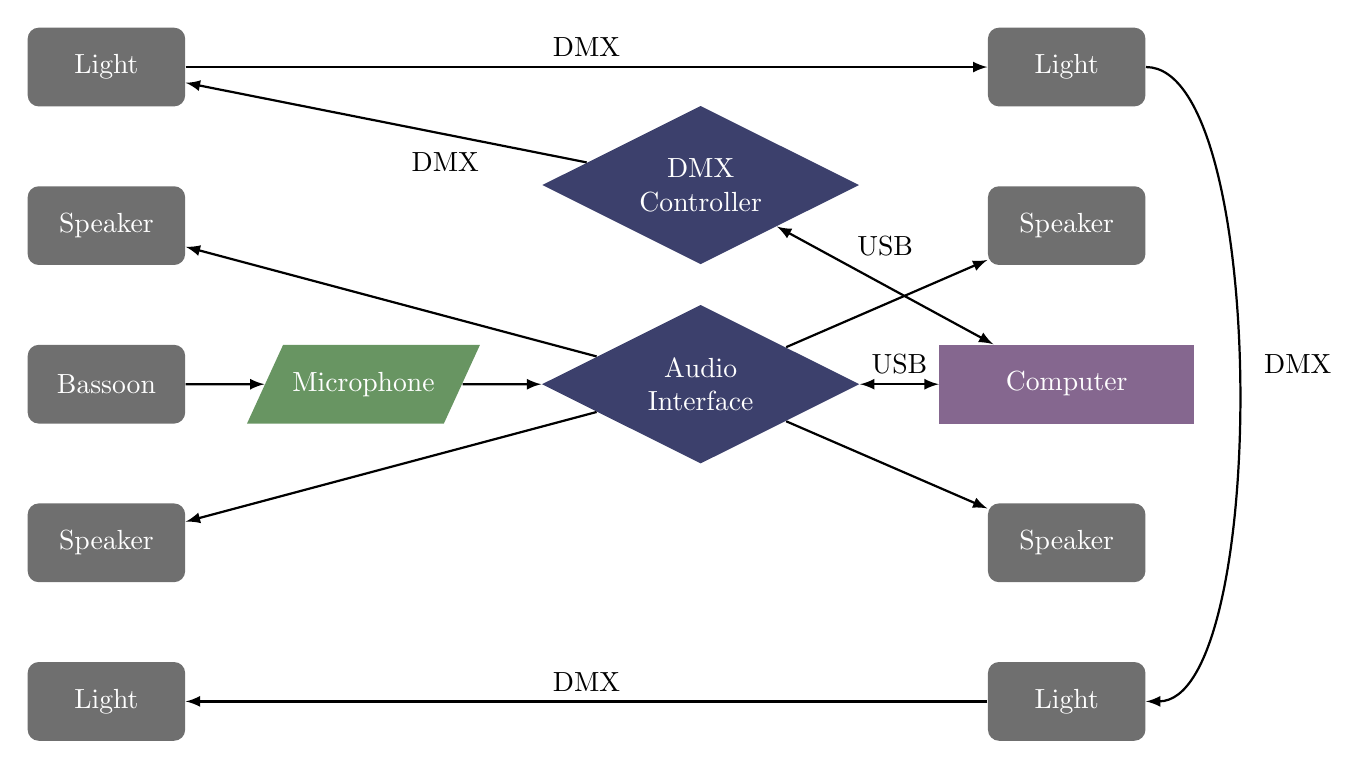
\begin{tikzpicture}[align=center,node distance = 1cm]
  \node (bsn) [source] {Bassoon};
  \node (mic1) [input, right= of bsn] {Microphone};
  \draw [cable] (bsn) -- (mic1);
  \node (interface) [routing, right= of mic1] {Audio Interface};
  \node (dmx) [routing, above = of interface, yshift = -0.5cm] {DMX Controller};
  \node (computer) [processor, text width = 3cm, right = of interface] {Computer};
  \draw [usb] (interface) -- node[anchor = south] {USB} (computer);
  \draw [usb] (computer) -- node[anchor=south, yshift=0.25cm] {USB} (dmx);
  \node (speaker1) [source, above = of computer] {Speaker};
  \node (speaker2) [source, below = of computer] {Speaker};
  \node (speaker3) [source, above = of bsn] {Speaker};
  \node (speaker4) [source, below = of bsn] {Speaker};
  \node (light1) [source, above = of speaker1] {Light};
  \node (light2) [source, below = of speaker2] {Light};
  \node (light3) [source, above = of speaker3] {Light};
  \node (light4) [source, below = of speaker4] {Light};
  \draw [cable] (interface) -- (speaker1);
  \draw [cable] (interface) -- (speaker2);
  \draw [cable] (interface) -- (speaker3);
  \draw [cable] (interface) -- (speaker4);
  \draw [cable] (mic1) -- (interface);
  \draw [cable] (dmx) -- node[anchor=south, xshift=0.75cm, yshift = -0.75cm] {DMX} (light3);
  \draw [cable] (light3) -- node[anchor=south] {DMX} (light1);
  \draw [cable] (light1) to[out = 0,looseness = 0.5, in = 0, looseness = 0.5] node[anchor=south, xshift = 0.75cm] {DMX} (light2);
  \draw [cable] (light2) -- node[anchor=south] {DMX} (light4);
\end{tikzpicture}


\end{document}
